\section{Supervisión de activos de Nebulas}

\label{supervision}

Como se muestra en la \figurename~\ref{fig:assets}, los activos de Nebulas se pueden dividir en: Activos Públicos Comunitarios y en Activos de la Fundación Nebulas.

\subsection{Activos Públicos Comunitarios}

\subsubsection{Composición}

\begin{itemize}
	\item 35 000 000 NAS (35\% del total en circulación): activos reservados para la comunidad tal como se declara en el \ntechw
    \item 8219,1744 NAS/día: a partir de consenso/generación de bloques e incluye:
	    \begin{itemize}
			\item 2\%: Consenso/Generación de bloques
			\item 1\%: Reserva de Fondos para el Desarrollo del Proyecto “Concejo de Nebulas”
		\end{itemize}
	\item 1\%(inicial): Incentivos propios para el \dip~\cite{mauvepaper}, desde el 13 de mayo de 2019
\end{itemize}

\subsubsection{Supervisión}

Los activos públicos pertenecen a la comunidad Nebulas; éstos se distribuyen automáticamente, son administrados mediante el proceso de gobernanza \onchain y son controlados por el Concejo de Nebulas.

\subsection{Activos de la Fundación Nebulas}

\subsubsection{Composición}

\begin{itemize}
	\item 20 000 000 NAS (20\%): Reserva del Equipo Nebulas tal como se establece en el \ntechw
    \item 5 000 000 NAS (5\%): Fondo para el Desarrollo de la Comunidad Nebulas (balance del \textit{Eco-investment Balance})
	\item Fondos iniciales de capital privado para el desarrollo del proyecto
	\item Ingresos por inversiones ecológicas iniciales
\end{itemize}

\subsubsection{Supervisión}

Los activos de la \fundneb son administrados por ese mismo organismo. La Fundación deberá velar para que la información sobre el uso de los activos sea abierta y transparente.

\begin{figure}
	\centering
	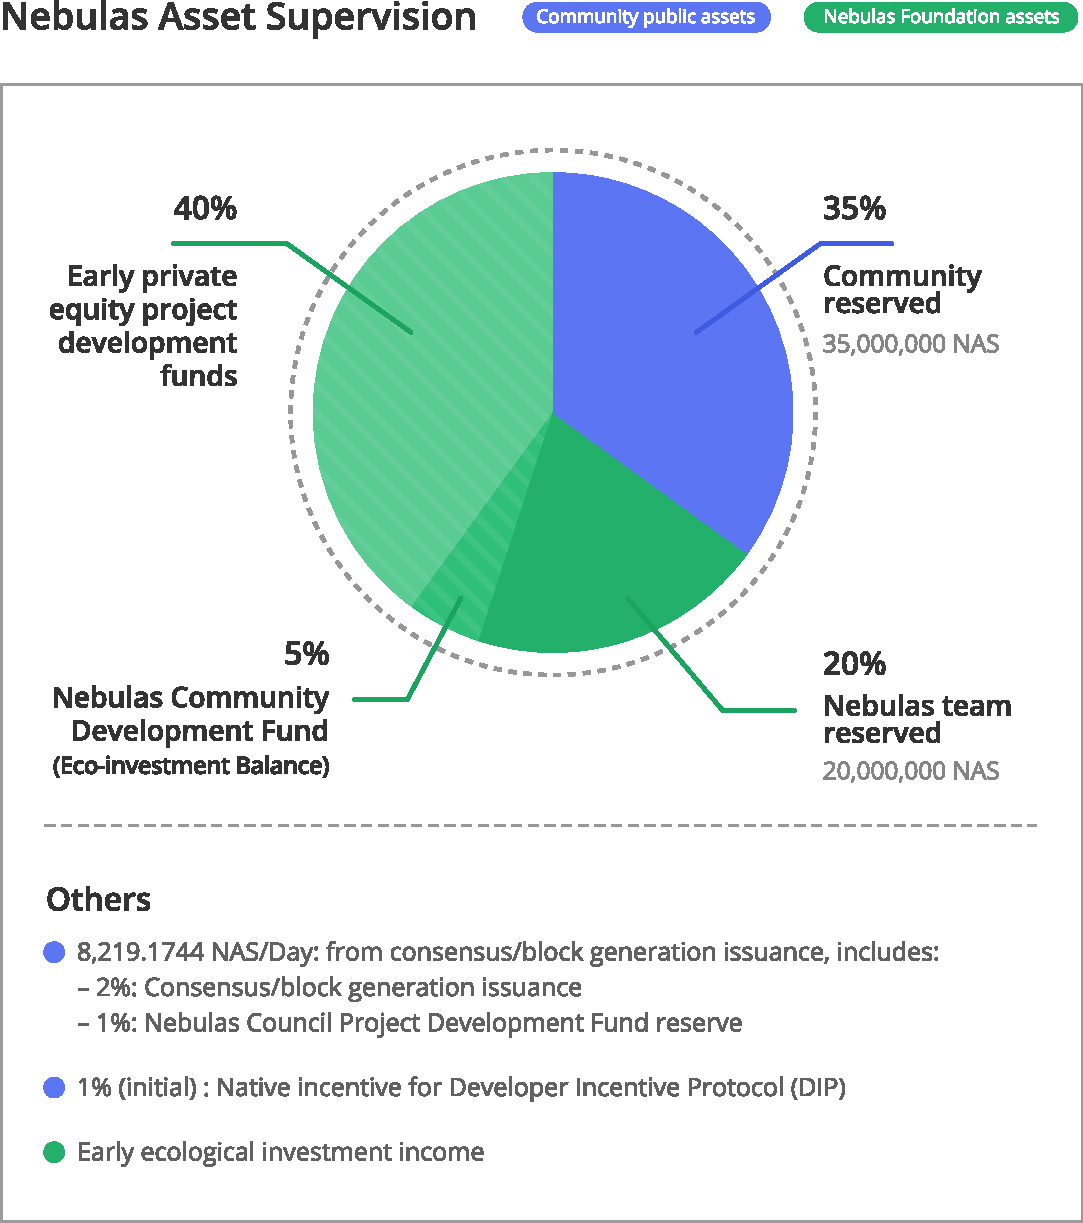
\includegraphics[width=1\textwidth]{../common/en/assets.pdf}
	\caption{Supervisión de activos en Nebulas \label{fig:assets}}
\end{figure}